\documentclass[twoside]{article}
\usepackage{amsgen,amsmath,amstext,amsbsy,amsopn,amssymb,color}
\usepackage{graphicx}
\usepackage{epsfig}

\setlength{\oddsidemargin}{0.1 in} \setlength{\evensidemargin}{-0.1
in} \setlength{\topmargin}{-0.6 in} \setlength{\textwidth}{6.5 in}
\setlength{\textheight}{10.5 in} \setlength{\headsep}{0.1 in}
\setlength{\parindent}{0 in} \setlength{\parskip}{0.1 in}

\newcommand{\red}{\textcolor{red}}

\newcommand{\homework}[2]{
   \pagestyle{myheadings}
   \thispagestyle{plain}
   \newpage
   \setcounter{page}{1}
   \noindent
   \begin{center}
   \framebox{
      \vbox{\vspace{2mm}
       \hbox to 6.28in { {\bf Math 4720:~Statistical Methods \hfill} }
       \vspace{6mm}
       \hbox to 6.28in { {\Large \hfill #1 (#2)  \hfill} }
       \vspace{6mm}
      \vspace{2mm}}
   }
   \end{center}
   \markboth{#1}{#1}
   \vspace*{4mm}
}

\newcommand{\bbF}{\mathbb{F}}
\newcommand{\bbX}{\mathbb{X}}
\newcommand{\bI}{\mathbf{I}}
\newcommand{\bX}{\mathbf{X}}
\newcommand{\bY}{\mathbf{Y}}
\newcommand{\bepsilon}{\boldsymbol{\epsilon}}
\newcommand{\balpha}{\boldsymbol{\alpha}}
\newcommand{\bbeta}{\boldsymbol{\beta}}
\newcommand{\0}{\mathbf{0}}

\begin{document}

\homework{$10^{th}$ and $11^{th}$ Week Summary}{04/03/25}
\vspace{-0.4 in}
\begin{itemize}
\item \textbf{ANOVA}\dotfill
\item Hypothesis Testing
\subitem $H_0: \mu_1 = \mu_2 = \cdots = \mu_t$
\subitem $H_a: \mu_i \neq \mu_j \;\; \text{for some pair } (i, j).$
\subitem Test Statistic: $F = \dfrac{{SSB}/{{df}_B}}{{SSE}/{{df}_E}}$
\subitem Decision Rule: Reject $H_0$ in favor of $H_a$ if $F > F_{\alpha}({df}_B, {df}_E)$.
\begin{figure}[h]
\begin{center}
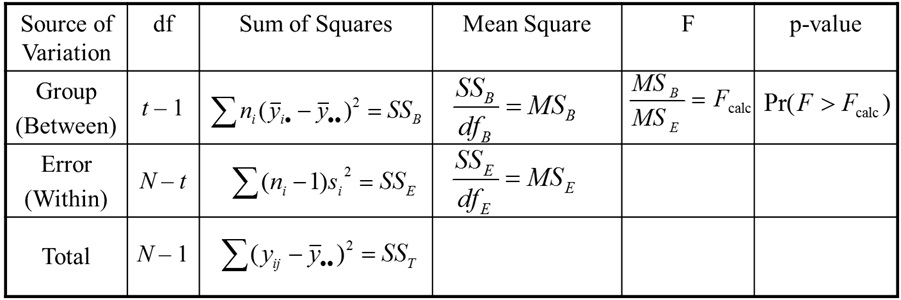
\includegraphics[angle=0, width=10.5 cm] {ANOVA_table.jpg}
\end{center}
\end{figure}
\vspace{-.25in}
\subitem R: \textsf{aov(Wt ~ sport + gender, data=ais2)}
\item For the above ANOVA table:
\subitem $N = \sum_{i} n_i$
\subitem ${SS_T} = {SS_B} + {SS_E}$
\subitem ${MS_E}$ is the pooled sample variance, an estimator for $\sigma^2$
\item Assumptions:
\subitem Homogeneity of variances: $\sigma_1 = \sigma_2 = \cdots = \sigma_t$.
\subitem Data are generated from normal distributions for each treatment.
\item What if normality fails?
\subitem We use the non-parametric test: ``Kruskal-Wallis Test''
\item What if the equality of variances fails?
\subitem We ``transform'' the data
\item What are the common transformations?
\subitem If $\sigma^2\propto\mu$, the use $Y_T=\sqrt{Y}$ or $\sqrt{Y+0.375}$
\subitem If $\sigma^2\propto\mu^2$, the use $Y_T=\ln(Y)$ or $\ln(Y+1)$
\subitem If $\sigma^2\propto\mu(1-\mu)$, the use $Y_T=\sin^{-1}\sqrt{Y}$
\item Assumptions for Oneway ANOVA model ($y_{ij}=\mu+\tau_i+\epsilon_{ij}$, where $i=1,\cdots,t$ and $j=1,\cdots,n_i$):
\subitem To test $H_0:\tau_i=0$ vs $H_a:\tau_i\neq0$ for some $i$:
\subitem (1) The $\epsilon_{ij}$'s are independent and normally distributed
\subitem (2) $\textrm{Var}(\epsilon_{ij})=\sigma^2$ (a constant value)
\item Checking the Assumptions:
\subitem Obtain the residuals ($r_{ij}=y_{ij}-\hat{\mu}-\hat{\tau}_i$) and fitted values ($\hat{y}_{ij}=\hat{\mu}+\hat{\tau}_i$), then
\subitem (1) The QQ-plot of $r_{ij}$'s should be linear
\subitem (2) The scatterplot of $r_{ij}$'s versus $\hat{y}_{ij}$'s should follow a random pattern.
\end{itemize}
\end{document}


